\item \points{1h}

In this question, you will train your policy gradient implementation on three different environments.

\begin{itemize}
	\item \href{https://www.gymlibrary.dev/environments/classic_control/cart_pole/}{CartPole-v1}
	\item \href{https://www.gymlibrary.dev/environments/mujoco/inverted_pendulum/}{InvertedPendulum-v4}
	\item \href{https://www.gymlibrary.dev/environments/mujoco/half_cheetah/}{HalfCheetah-v4}
\end{itemize}

For each of the 3 environments, choose 3 random seeds and run your policy gradient implementation both with and without a baseline.

\clearpage
\textbf{Training Policy Gradient}

The general form for running your policy gradient implementation is as follows (where config\_filename is the name of a yaml file in the ~src/config~ folder with your training configuration):

\begin{lstlisting}
$ python run.py --config_filename config_filename
\end{lstlisting}

Depending on the configuration file details you provide this command may train models for more than one seed which can take a while (especially for \textit{HalfCheetah-v4}). As a result, you may wish to run these jobs as background processes in which case you may run the command as follows:

\begin{lstlisting}
$ nohup python run.py --config_filename config_filename &
\end{lstlisting}

This will prevent the python process from ending when you close your terminal window as well as running the command in the background. Additionally, in the directory where you run the command a ~nohup.out~ file is created and contains the standard output from the process that you are running. Feel free to make use of this form of the command for the longer running processes.

\textbf{Altering the Training Configuration}

We have provided you with sample configuration files in the assignment ~config~ folder for you to use such as ~config/cartpole_baseline.yml~. These configurations will be suitable to use directly in training your agent without altering the config file.

However, you may optionally alter the training configuration files directly to run your policy gradient implementation with different settings. Below we have briefly described some of the changes you could apply:

\begin{itemize}
\item To run your implementation with/without a baseline you may change the ~use_baseline~ option to either ~true~ or ~false~.

\item You may also choose to train multiple seeds under the one python process through specifying more than one seed in the list ~seed~ (equally you may specify a single seed in this list if you want to run just one).

\item You may also wish to qualitatively observe the performance of your agent. To do so, you can record a single episode of the trained agent through changing the ~record~ option to ~true~ in the training configuration file for your run. Once your training run is complete you should see a video recording outputted in the ~results~ folder for the given run.
\end{itemize}

\textbf{Results \& Plotting}

Once training is complete you should observe the creation of the following folder ~src/results~ which contains the results of your training runs. In addition, you should note that some files based on model evaluation have been created in the submission folder. This contains the weights and scores for one of your training runs for each environment and baseline/no baseline configuration (this will only populate once one of your training runs achieves evaluation scores above a certain threshold). You will need to upload these weights with your submission to receive full credit for this question. To plot your results for certain seeds run:

\begin{lstlisting}
$ python run.py --plot_config_filename plot_config_filename
\end{lstlisting}

where plot\_config\_filename is the name of a yaml file in the ~src/config~ folder containing information on the seeds we wish to plot and for which environments. Please consult ~config/plot.yml~ for an example of the structure of this configuration file.

On the following page we provide sample outputs and an outline of the performance you can expect for the correct implementation.

\clearpage
\textbf{Expected Results}

We expect your plots to look similar to the plots which we have included:

\begin{figure}[H]
\centering
  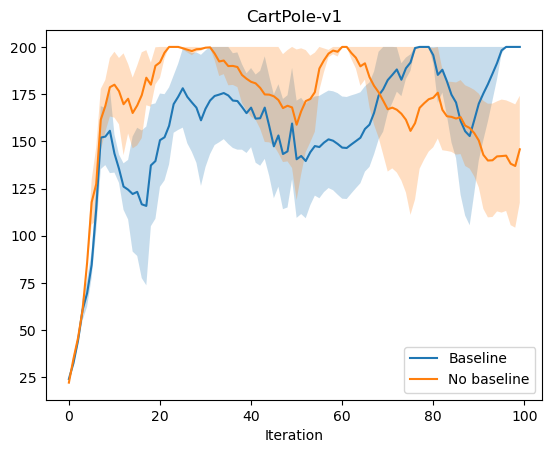
\includegraphics[width=.45\linewidth]{images/CartPole-v1.png}
  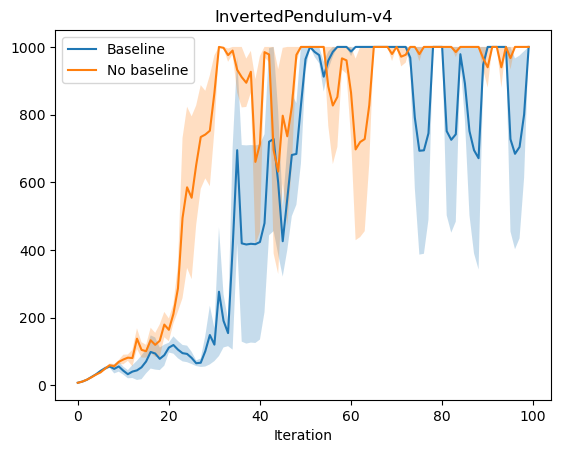
\includegraphics[width=.45\linewidth]{images/InvertedPendulum-v4.png}
\end{figure}

\begin{figure}[H]
\centering
  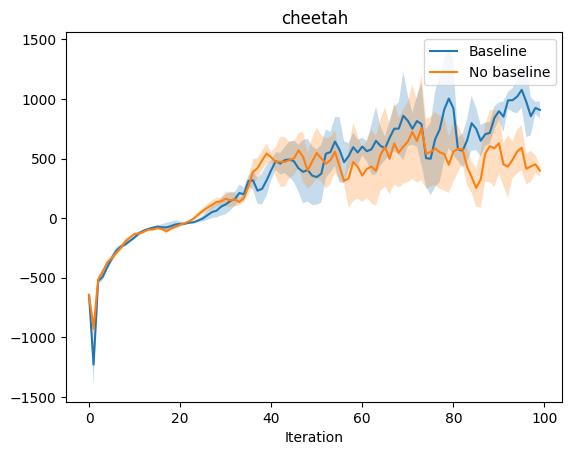
\includegraphics[width=.45\linewidth]{images/HalfCheetah-v4.png}
\end{figure}

The following performance benchmarks need to be achieved by your implementation in order to receive full credit for this question:

\begin{itemize}
	\item CartPole-v1: agent should reach the maximum return of 200 with and without baseline (although it may not stay there)
	\item InvertedPendulum-v4: agent should reach the maximum return of 1000 with and without baseline (although it may not stay there)
	\item HalfCheetah-v4: agent should reach at least a score of 200 with and without baseline (in general it can achieve a much higher score e.g. 900)
\end{itemize}
\clearpage
